% !Mode:: "TeX:UTF-8"
%%% Local Variables:
%%% mode: latex
%%% TeX-master: t
%%% End:

\chapter{深度学习相关理论}
\label{cha:chap02}
深度学习是以人工神经网络为架构,通过多隐层网络结构提取高层抽象特征,对数据进行表征学习的算法。常见的深度学习框架包含深度神经网络(Deep neural network, DNN)、深度置信网络(Deep belief network, DBN)、递归神经网络(Recurrent neural network, RNN)和卷积神经网络(Convolutional neural network, CNN)等\cite{krizhevsky2012imagenet} 。 与其他网络结构相比,CNN 利用输入数据的二维结构信息,在图像分类与识别、图像语义分割等视觉任务中能够给出更好的结果。
%%

\section{卷积神经网络基础}
\label{sec:chap02-1}

% 深度前馈神经网络
CNN 是一种带有卷积结构的深度前馈神经网络,使用反向传播(Backpropagation,BP)算法进行权值更新,主要用于图像分类与识别。CNN 网络结构一般由卷积层(Convolutional layer)、池化层(Pooling layer)和全连接层(Full connected layer)交叉堆叠而成。卷积层和池化层用于提取图像高阶特征,具有局部连接、权值共享和下采样等特性。全连接层可以看作CNN 分类网络的决策分类器,将学到的“分布式特征表示”映射到样本标记空间。。
%全连接层起到图像“分类器”的作用,将学到的“分布式特征表示”映射到样本标记空间。
%卷积层(Convolutional layer)、池化层(Pooling layer)和全连接层(Full connected layer)

\subsubsection*{1. 卷积层}
\label{subsec:chap02-2-1-1}
卷积(Convolution)是分析数学中的一种运算,被广泛应用到信号处理与图像处理中。因为图像是两维结构数据,图像处理中常用二维卷积运算。给定一个图像$X \in \mathbb{R}^{M \times N}$,和滤波器$W \in \mathbb{R}^{m \times n}$, 一般满足$m \ll M, n \ll N$,其卷积输出:
\begin{equation}
  \label{eq:2-15}
  Y = X \otimes W
\end{equation}
式中,$\otimes$ 是卷积运算。 输出特征图上某点$(i,j)$ 的值可由式\ref{eq:2-16}计算得到:
\begin{equation}
  \label{eq:2-16}
  y_{ij} = \sum_{u=1}^m\sum_{v=1}^n w_{uv}\cdot x_{i-u+1,j-v+1}
\end{equation}

CNN 最核心结构是卷积层,每个卷积层均包含一个或多个二维平面,该二维平面称作CNN 网络的特征图(Feature map)。卷积层中的神经元共享权重,CNN 中共享的权重称为卷积核(Convolutional kernel),卷积核对上层特征图进行卷积操作提取影像特征。如图~\ref{fig:conv_op} 所示,图中使用大小为$3\times3$的卷积核,输入图像大小为$5\times5$,卷积核从左上方以$1$ 个像素点的步长(Stripe)开始滑动,图像中像素点与卷积核之间卷积运算后的输出到特征图上的对应位置。

% 同一特征图内神经元共享权重和偏置项,且每一个神经元与上一层的区域局部连接
% 利用卷积核对上一层的特征图进行卷积运算可以提取影像特征产生下一层网络的输出层。

\begin{figure}[htbp]
  \centering
  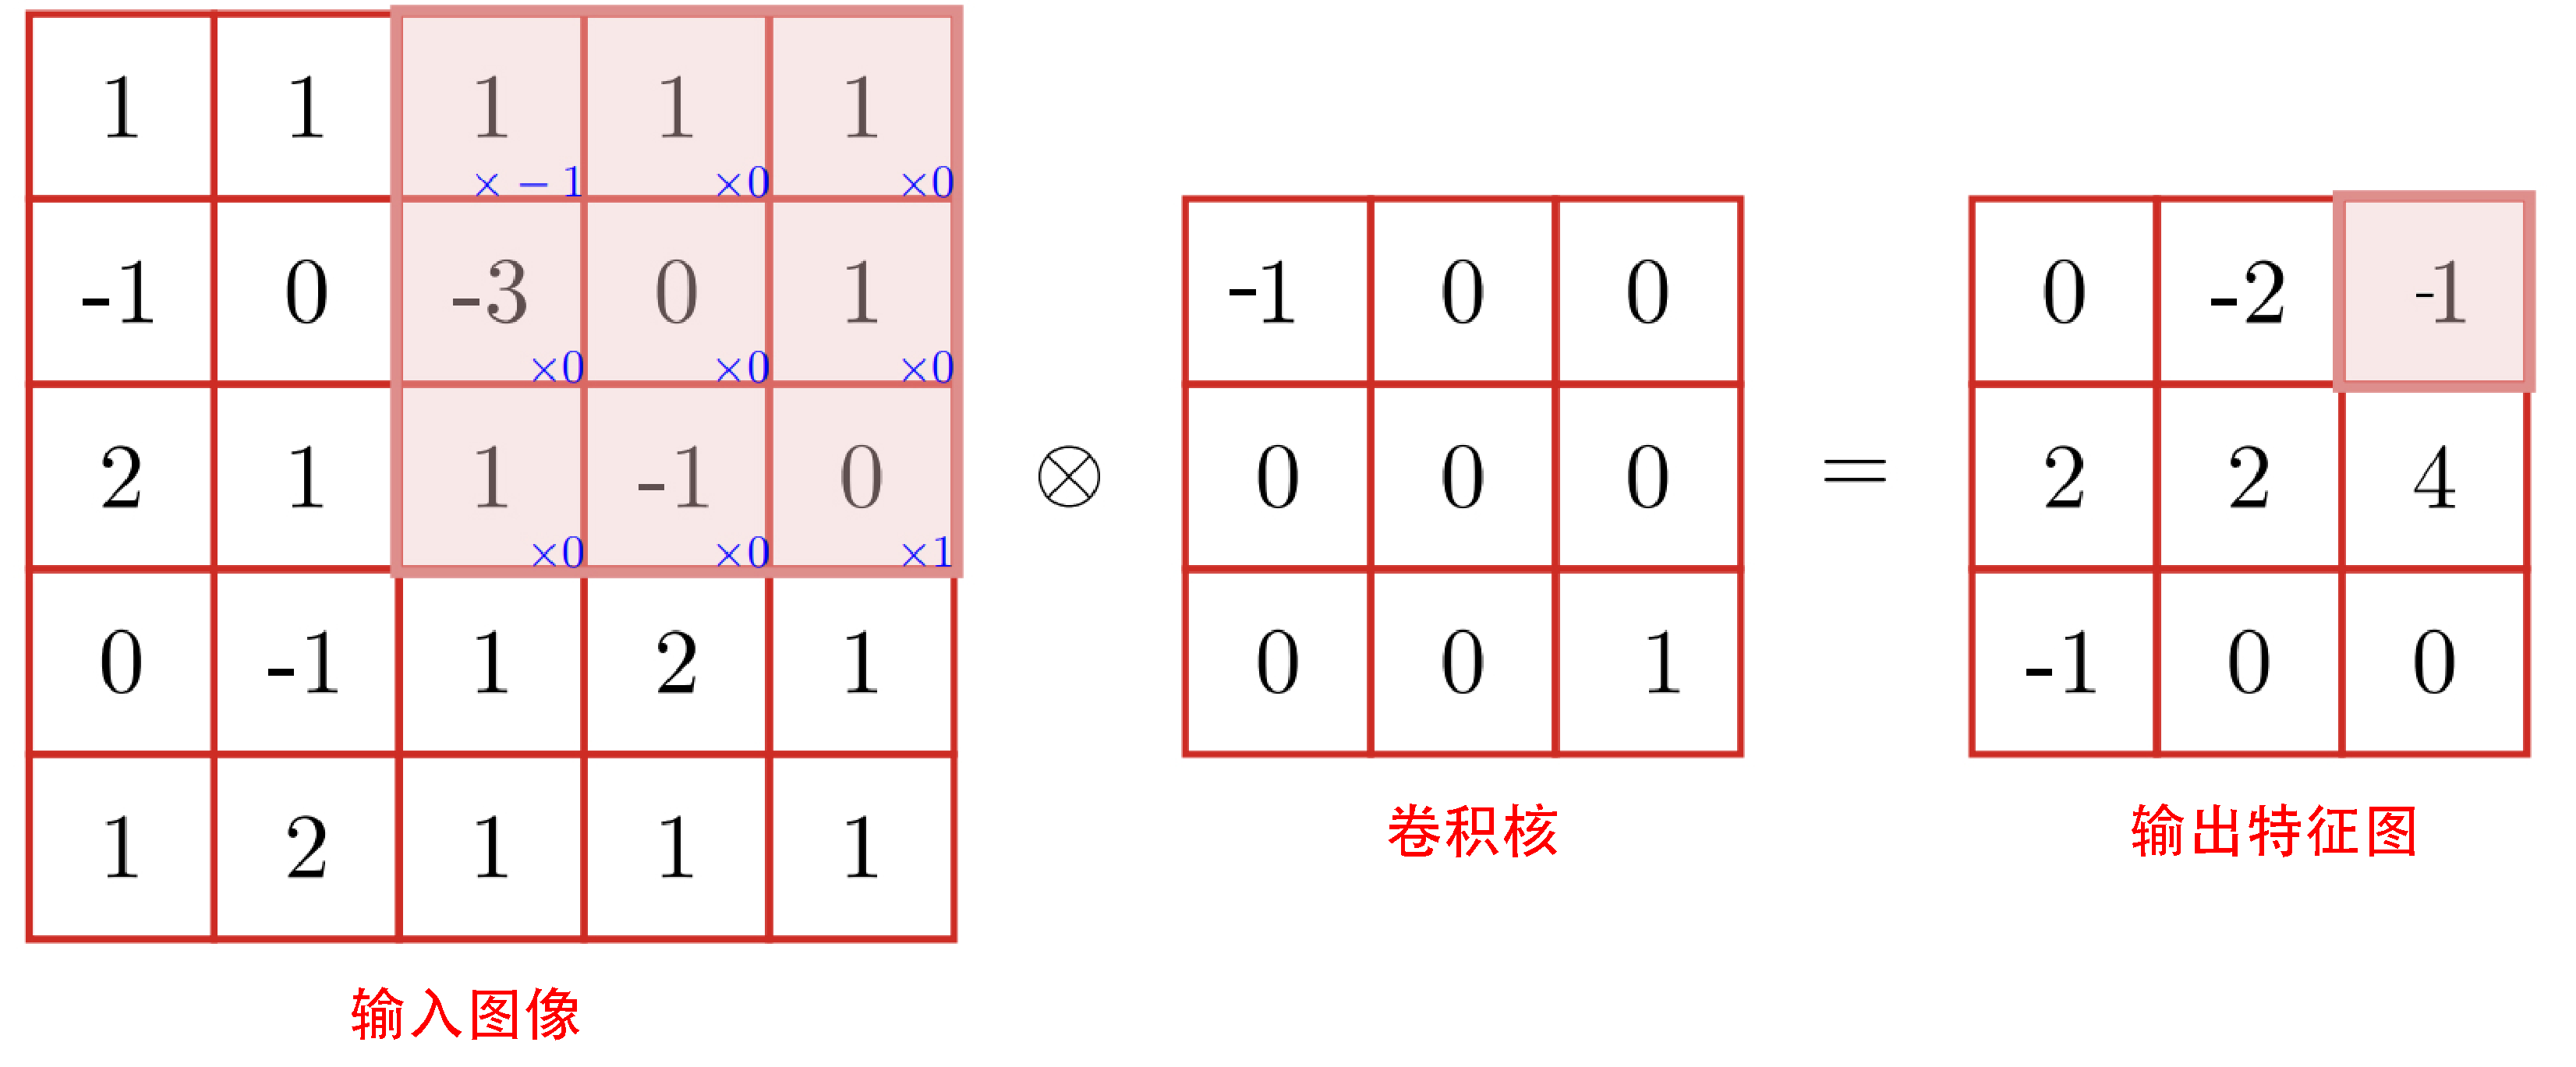
\includegraphics[width=0.8\textwidth]{figures/conv_op}
  \caption{图像卷积示意图}\label{fig:conv_op}
\end{figure}

图像卷积运算时,与全连接模式中每个像素点对应一个独立的计算权值不同,所有位置的输出神经元均使用一个卷积核计算权值,这样做的好处是既减少参数的数量,又利用了图像特征的局部性特点。图像卷积中,每个卷积核都可以提取图像的一种特征,所以一般设置多个卷积核,利用不同的卷积核来提取图像不同的特征。

卷积计算中第$l$ 层的输入是第$l-1$ 层的卷积输出特征图,假定第$l-1$ 层输入大小为$X_{l-1} \times X_{l-1}$,卷积核大小为$K \times K$,滑动步长为$S$,边界填充(Padding)大小为$P$,$l-1$ 层的输出特征图(即第$l$ 层的输入)的大小为$X_l \times X_l$,可由式\ref{eq:2-17} 计算得到:
\begin{equation}
  \label{eq:2-17}
  X_l = \lfloor \frac{X_{l-1} - K + 2 \times P}{S} \rfloor + 1
\end{equation}

卷积操作是线性的,即使联合多个线性模型输出依旧是线性的。实际识别任务往往是复杂、非线性的,线性神经网络实用性不强。如果为每个卷积输出加一个非线性函数,神经网络模型就不再是线性的,这个非线性函数就是激活函数。常用的激活函数有Sigmoid、TanHyperbolic(tanh) 和线性整流函数(Rectified linear unit, ReLU) 函数等。当前卷积网络常用的是ReLU 激活函数,ReLU 函数表达式如下:
\begin{equation}
  \label{eq:2-17-1}
  f(x) = \max(x,0)
\end{equation}
相比Sigmoid 和tanh 函数,ReLU 对于梯度训练的收敛有巨大加速作用,反向传播训练时不易饱和,另外ReLU 函数简单,运算量很小,因此广泛使用到卷积网络非线性激活中。

\subsubsection*{2. 池化层}
\label{subsec:chap02-2-1-2}
池化层又叫下采样层(Subsampling layer),能够缩小特征图尺寸,其作用是进行特征选择,降低特征数量,使特征更加抽象。卷积层虽然可以大幅减少网络参数的数量,但并没有显著减少特征映射组中神经元的个数。在卷积层后面加上一个池化层,可以减少网络下一层的数据量,实现特征降维,一定程度上防止过拟合。

假定池化层的输入特征图为$X \in \mathbb{R}^{M \times N}$ ,将其划分为很多区域$R_{m,n},1 \leq m \leq M, 1 \leq n \leq N$,这些区域可以重叠,也可以不重叠。池化层通过池化函数对特征图的每个区域$R_{m,n}$ 进行下采样,得到一个值作为这个区域的概括。根据采样的方式不同,常用的池化函数有两种:
\begin{enumerate}[1. ]
  \label{list:1}
  \item 最大池化(Maximum pooling)
        最大池化是将区域内所有神经元的最大值作为池化层输出。
        \begin{equation}
          \label{eq:2-18}
          Y_{m,n} = \mathop{\max}_{i \in R_{m,n}} x_i
        \end{equation}
        其中,$x_i$ 为区域$R_k$ 内每个神经元的激活值。

  \item 平均池化(Average pooling)
        平均池化是选取区域内所有神经元激活值的和的平均值。
        \begin{equation}
          \label{eq:2-19}
          Y_{m,n} =  \frac{1}{|R_{m,n}|}\mathbb{\sum}_{i \in R_{m,n}} x_i
        \end{equation}
\end{enumerate}
对输入特征图的所有区域进行下采样,就可以得到池化层的输出特征图$Y = \{ Y_{m,n}\},1 \leq m \leq M, 1 \leq n \leq N$ 。

\begin{figure}[htbp]
  \centering
  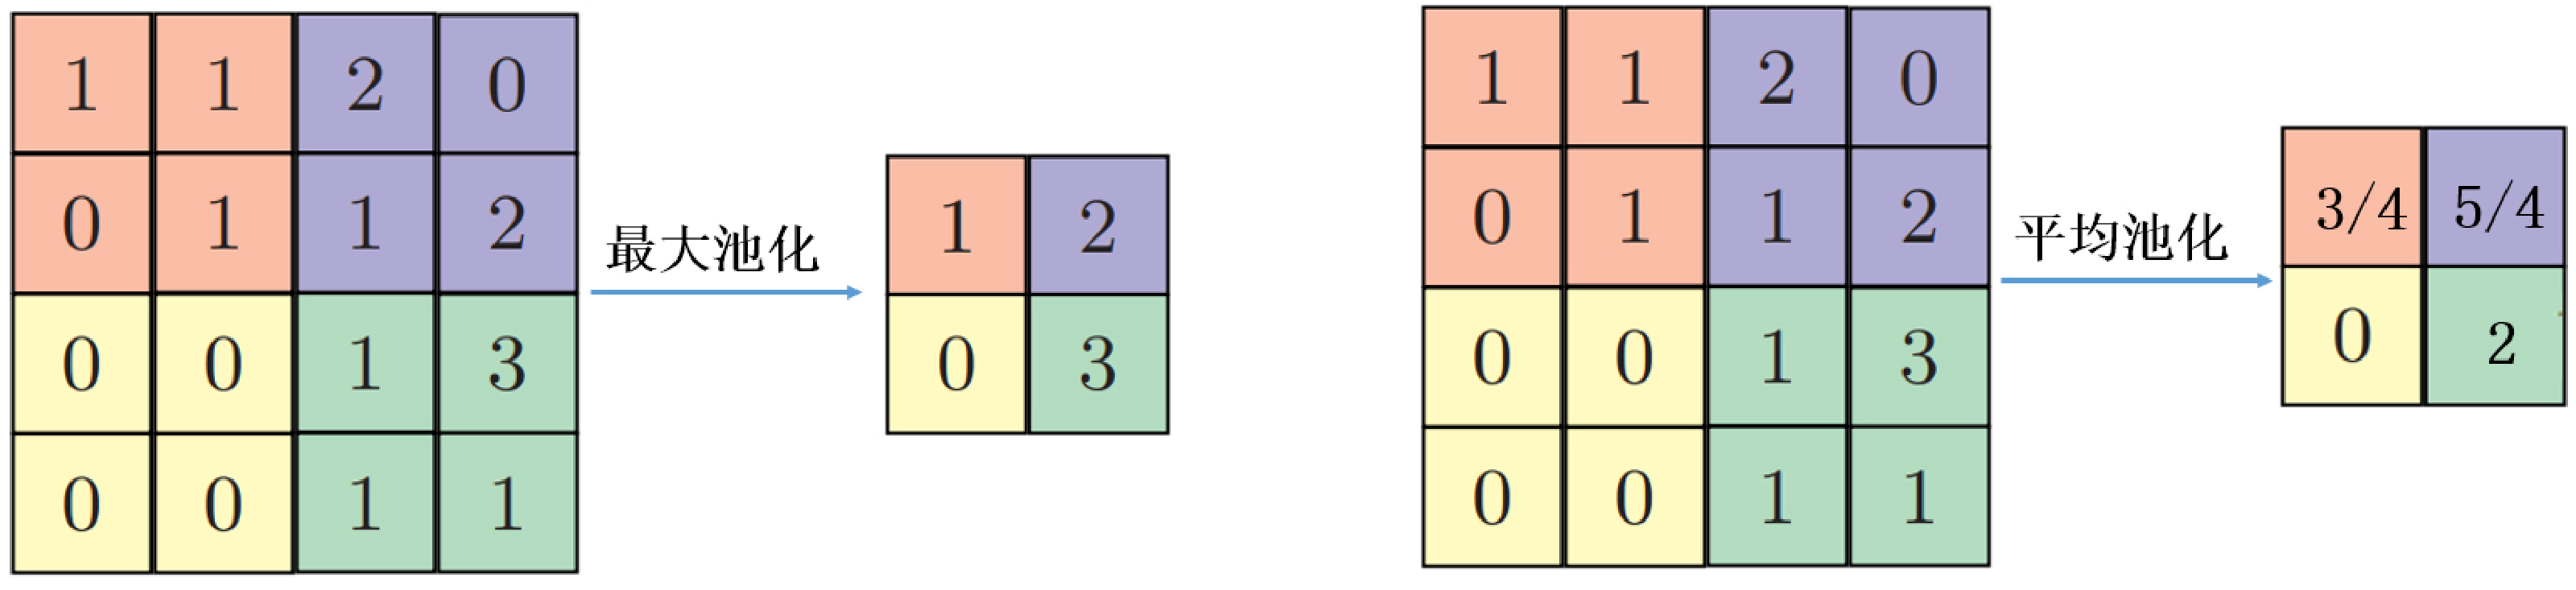
\includegraphics[width=0.9\textwidth]{figures/pooling}
  \caption{最大池化与平均池化}\label{fig:pooling}
\end{figure}

图如~\ref{fig:pooling} 所示,输入特征图大小为$4 \times 4$,池化函数核为$2 \times 2$,滑动步长为$2$ ,分别进行最大池化和平均池化操作,得到不同的池化输出特征图。

在卷积网络的最后,往往会接入一两层的全连接层。全连接层将卷积输出的二维特征“拍平”,转化成一个一维向量。全连接层对卷积输出特征高度提取,方便交给最后的分类器(如SVM 分类器、Softmax 分类器等)实现图像分类。

\subsubsection*{3. 典型的卷积网络结构}
\label{subsec:chap02-2-1-3}
% 一个典型的卷积网络由卷积层、池化层和全连接层交叉堆叠而成。
一个典型的卷积网络由卷积层、池化层和全连接层交叉堆叠而成。如图~\ref{fig:cnn_structure} 所示,通常一个卷积块由连续的$M$ 个卷积层和$b$ 个池化层拼接而成($M$ 一般取$1\sim 4$,$b$ 可取$0$或$1$), 一个完整的用于分类任务的卷积网络结构通常由$N$ 个堆叠的卷积块后接$K$ 个全连接层组成($N$ 一般取$1\sim 100$,$K$ 取$1 \sim 2$)。CNN 中多层网络模型使得网络模型对不同形态的图像具有优秀的适应能力,它可以自动学习高分影像中复杂的特征,提升影像分类精度。
%它可以拟合高分影像中因地物尺度不一、拍摄角度不同等原因形成的复杂特征,从而有效提高分影像的分类识别精度。

\begin{figure}[htb]
  \centering
  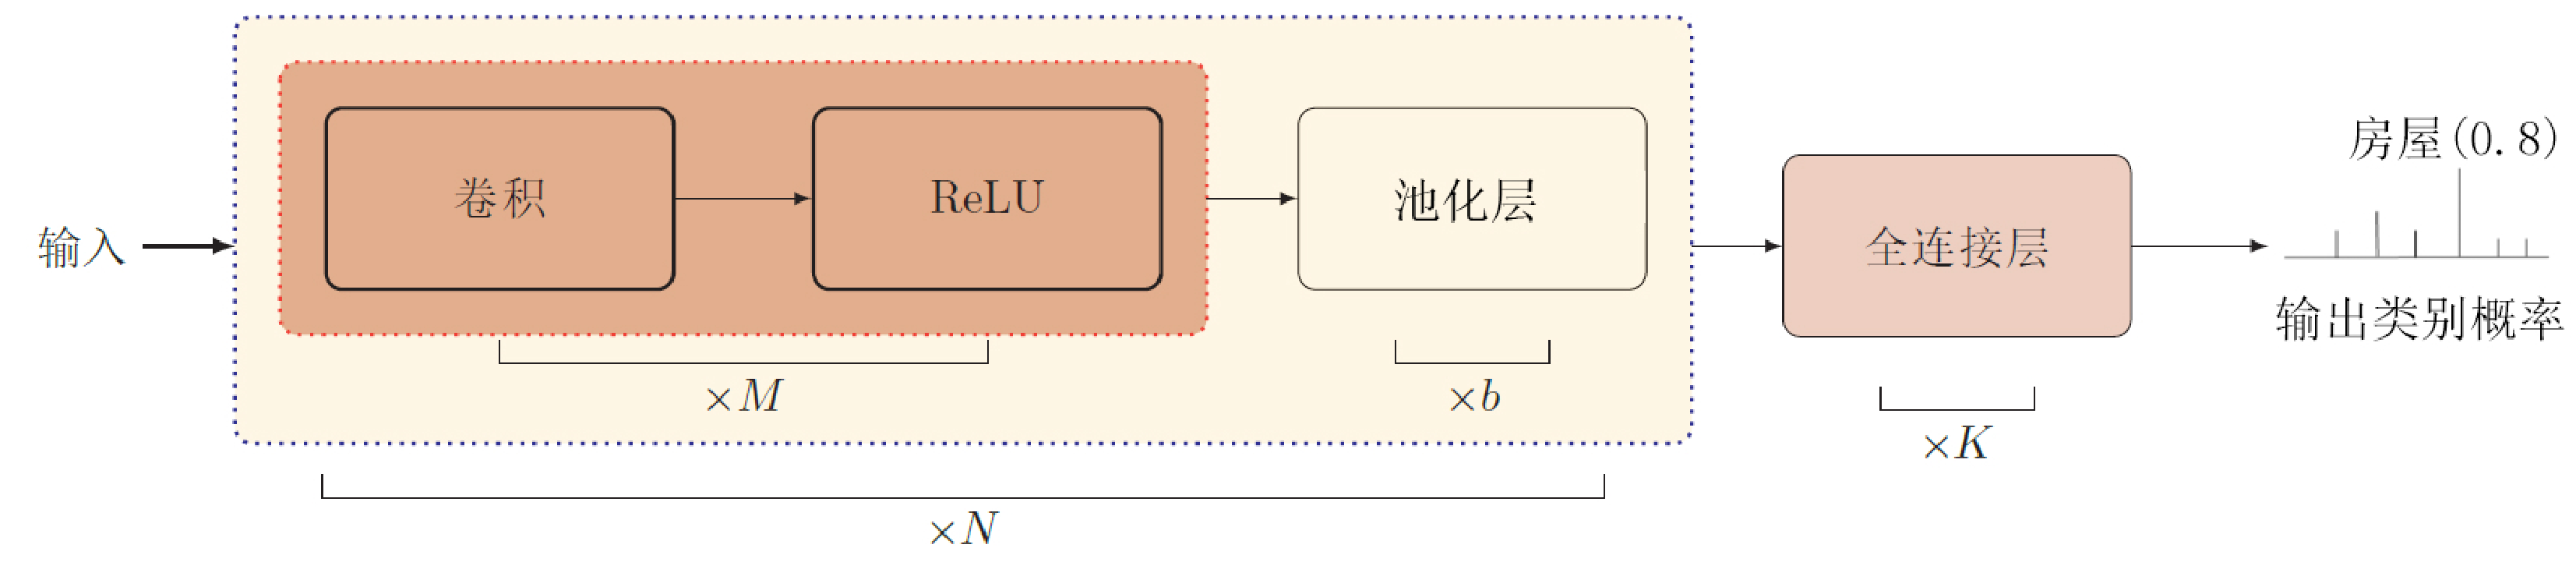
\includegraphics[width=1.0\textwidth]{figures/cnn_structure}
  \caption{典型的卷积网络结构}\label{fig:cnn_structure}
\end{figure}

\section{全卷积神经网络}
\label{ssec:chap02-2}
经典的CNN 模型最右端结构通常为全连接层,它会将原来二维影像映射到一维空间,因而会失去二维图像的空间位置信息,且网络输出常为输入图像属于某一类别的概率。与分类对整张图片类别预测不同,图像的语义分割是对目标图像的每个像素点进行分类,即语义分割是从像素级对图像进行类别预测。全卷积神经网络(Fully convolutional network,FCN)\cite{long2015fully} 由Jonathan Long 等人于2016年提出,其创造性地利用卷积层替代分类网络中的全连接层,进而保证网络输出为二维的分类结果图,使用反卷积(Deconvolution)的上采样策略,得到一个与原图尺寸大小相同的分割图,实现图像像素级的分类预测。图像语义分割引入遥感分类领域即为遥感影像分类。图~\ref{fig:fcn_structure} 为遥感影像分类的全卷积网络结构示意图,全卷积网络将学习到的遥感影像判别特征解码映射到高分辨率空间,完成影像的像素级分类。

\begin{figure}[htb]
  \centering
  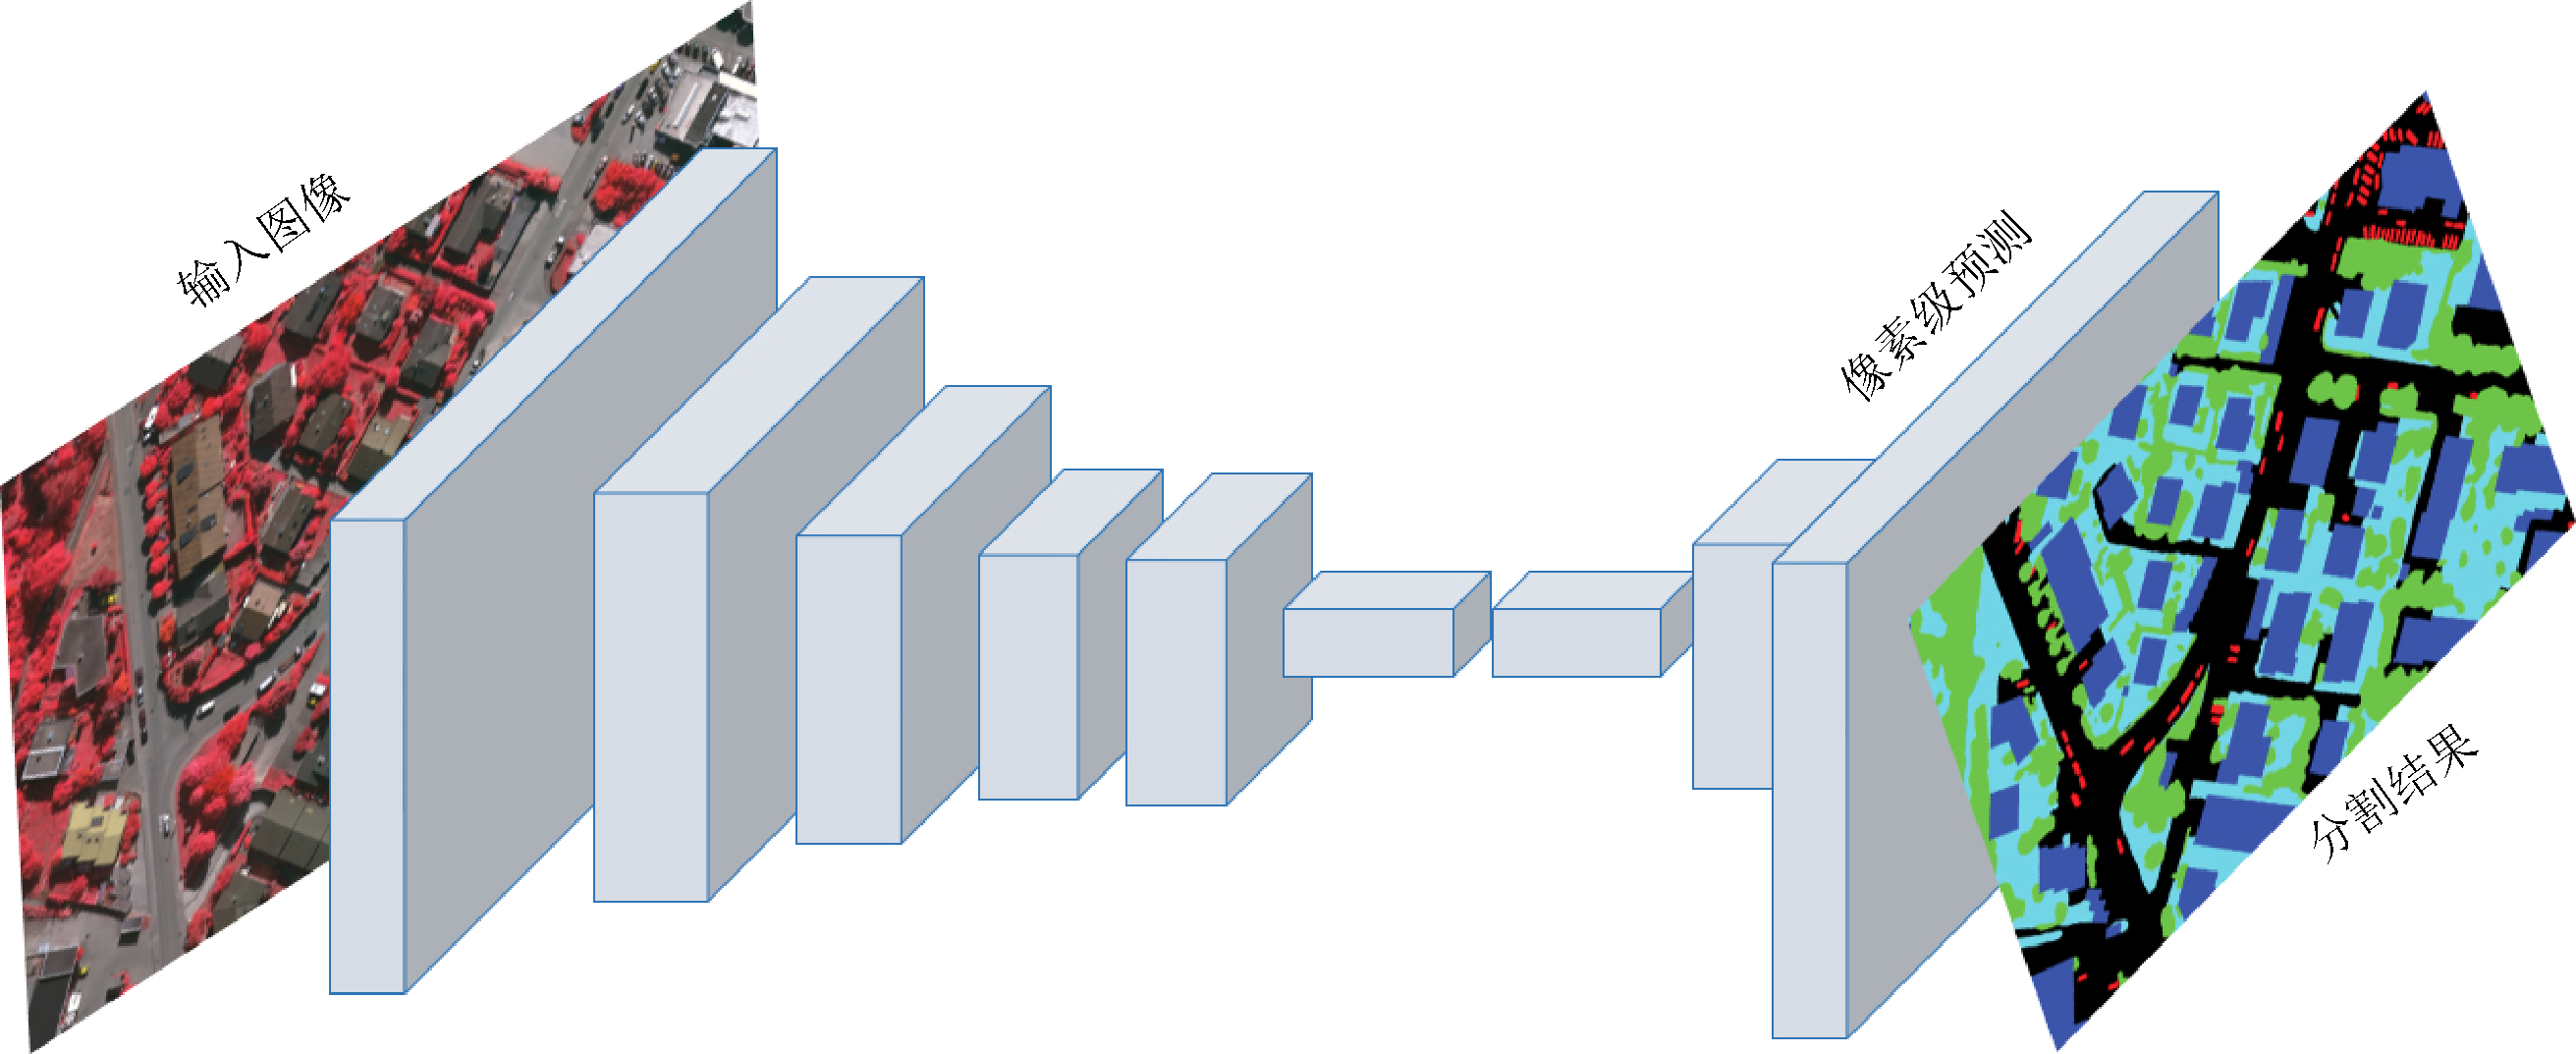
\includegraphics[width=0.9\textwidth]{figures/FCN}
  \caption{影像分类网络结构示意图}\label{fig:fcn_structure}
\end{figure}

\subsubsection*{1. 反卷积}
\label{subsec:chap02-2-2-1}
反卷积,又叫转置卷积,是一种上采样操作,可以理解为下采样的逆过程。卷积运算是一个下采样过程,一般通过卷积操作实现高维特征到低维特征的转换。如对输入$4\times 4$ 的二维特征,用大小$3\times 3$ 的核,做步长为$1$ 的卷积运算得到$2\times 2$ 的特征输出。反卷积则实现低维特征到高维特征的转换。与之对应,反卷积对输入为$2\times 2$ 的二维特征,使用$3\times 3$ 的核操作得到$4\times 4$ 的输出。如图~\ref{fig:deconv} 所示,输入特征大小$2\times 2$,核大小$3\times 3$,步长$s=1$,填充补0为$p=2$,经过反卷积处理输出尺寸上采样到$4\times 4$, 图中显示了反卷积上采样的计算过程。

\begin{figure}[htb]
  \centering
  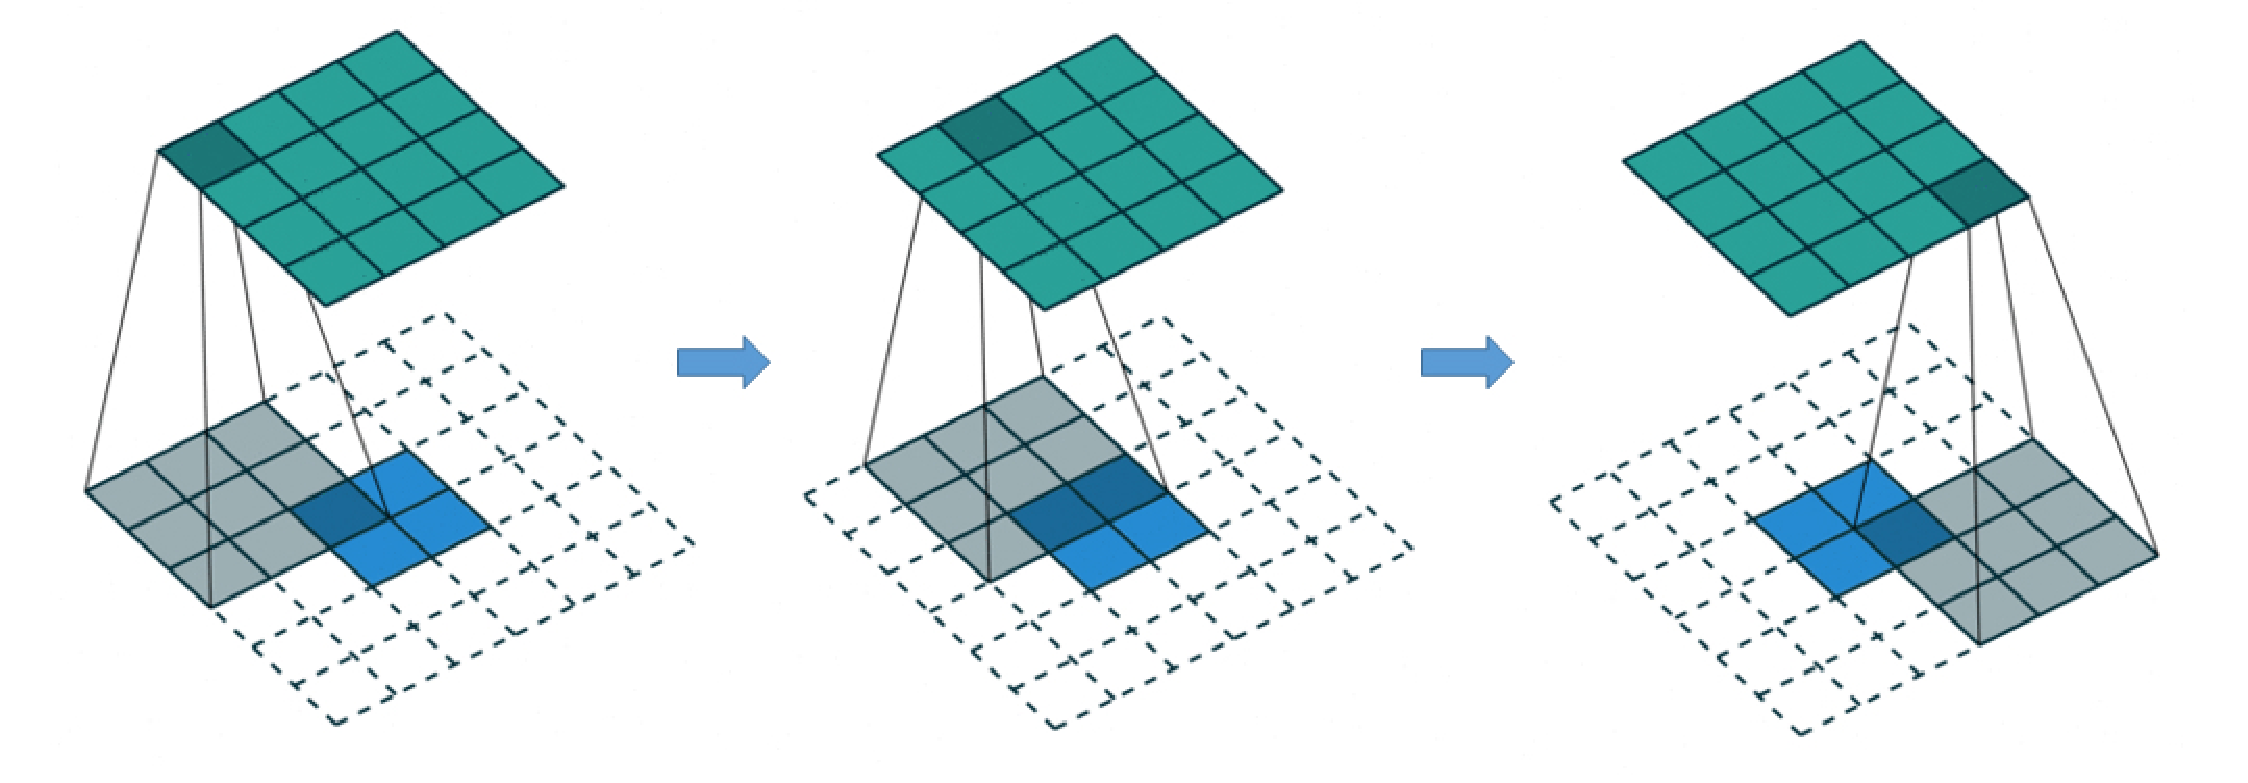
\includegraphics[width=0.8\textwidth]{figures/deconv}
  \caption{反卷积上采样过程}\label{fig:deconv}
\end{figure}

反卷积是卷积运算形式上转置的映射关系。对一个大小为$X\times X$的图像$\textit{I}$,和大小为$K\times K$ 的卷积核,进行步长为$S \geq 1$ 的反卷积运算,先对图像$\textit{I}$ 进行两端补零$P=K-1$,并且在每两个像素间填充$S-1$ 个$0$,最后进行步长为$1$ 的卷积操作,得到反卷积的输出结果,设输出特征维度为$O \times O$ ,满足:
\begin{equation}
  \label{eq:2-20}
  O = S \times (X - 1) + K
\end{equation}

\subsubsection*{2. 基于FCN 影像分类}
\label{subsec:chap02-2-2-2}
FCN 网络由卷积特征提取和反卷积上采样两部分组成。FCN 特征提取阶段,为了加快网络训练速度,常使用在ImagaNet 等数据集上训练好的网络权值初始化FCN 网络参数,如对训练好的AlexNet\cite{krizhevsky2012imagenet} 或VGG\cite{simonyan2014very} 网络权值,选取除全连接层的权值参数初始化FCN 网络。输入图片经卷积池化层处理后特征图尺寸变小,所以特征图需要被上采样为输入图片相同尺寸。FCN 使用反卷积层做上采样将特征图尺寸调整为原输入图像大小。 同时,为了得到更精细的分类结果,FCN 中使用跳层连接(Skip connections)将下采样阶段和上采样阶段相同尺寸的特征图融合。图~\ref{fig:vgg-fcn} 为基于FCN 网络结构影像分割示意图。图中虚线上半部分为卷积池化网络结构,模型使用训练好的VGG 16 网络权值(去除全连接层权值)初始化,堆叠的卷积层与池化层能够确保提取影像数据高阶特征。图中虚线下半部分,分别从卷积网络的不同阶段预测网络的分类结果,利用反卷积层对最后一个卷积层特征图上采样处理,使特征图尺寸还原为原始输入影像大小,保留了原始输入图像中的空间信息,从而对每一个像素都产生了一个预测,最后在上采样的特征图上进行逐像素分类,完成FCN 网络的图像语义分割。

\begin{figure}[htb]
  \centering
  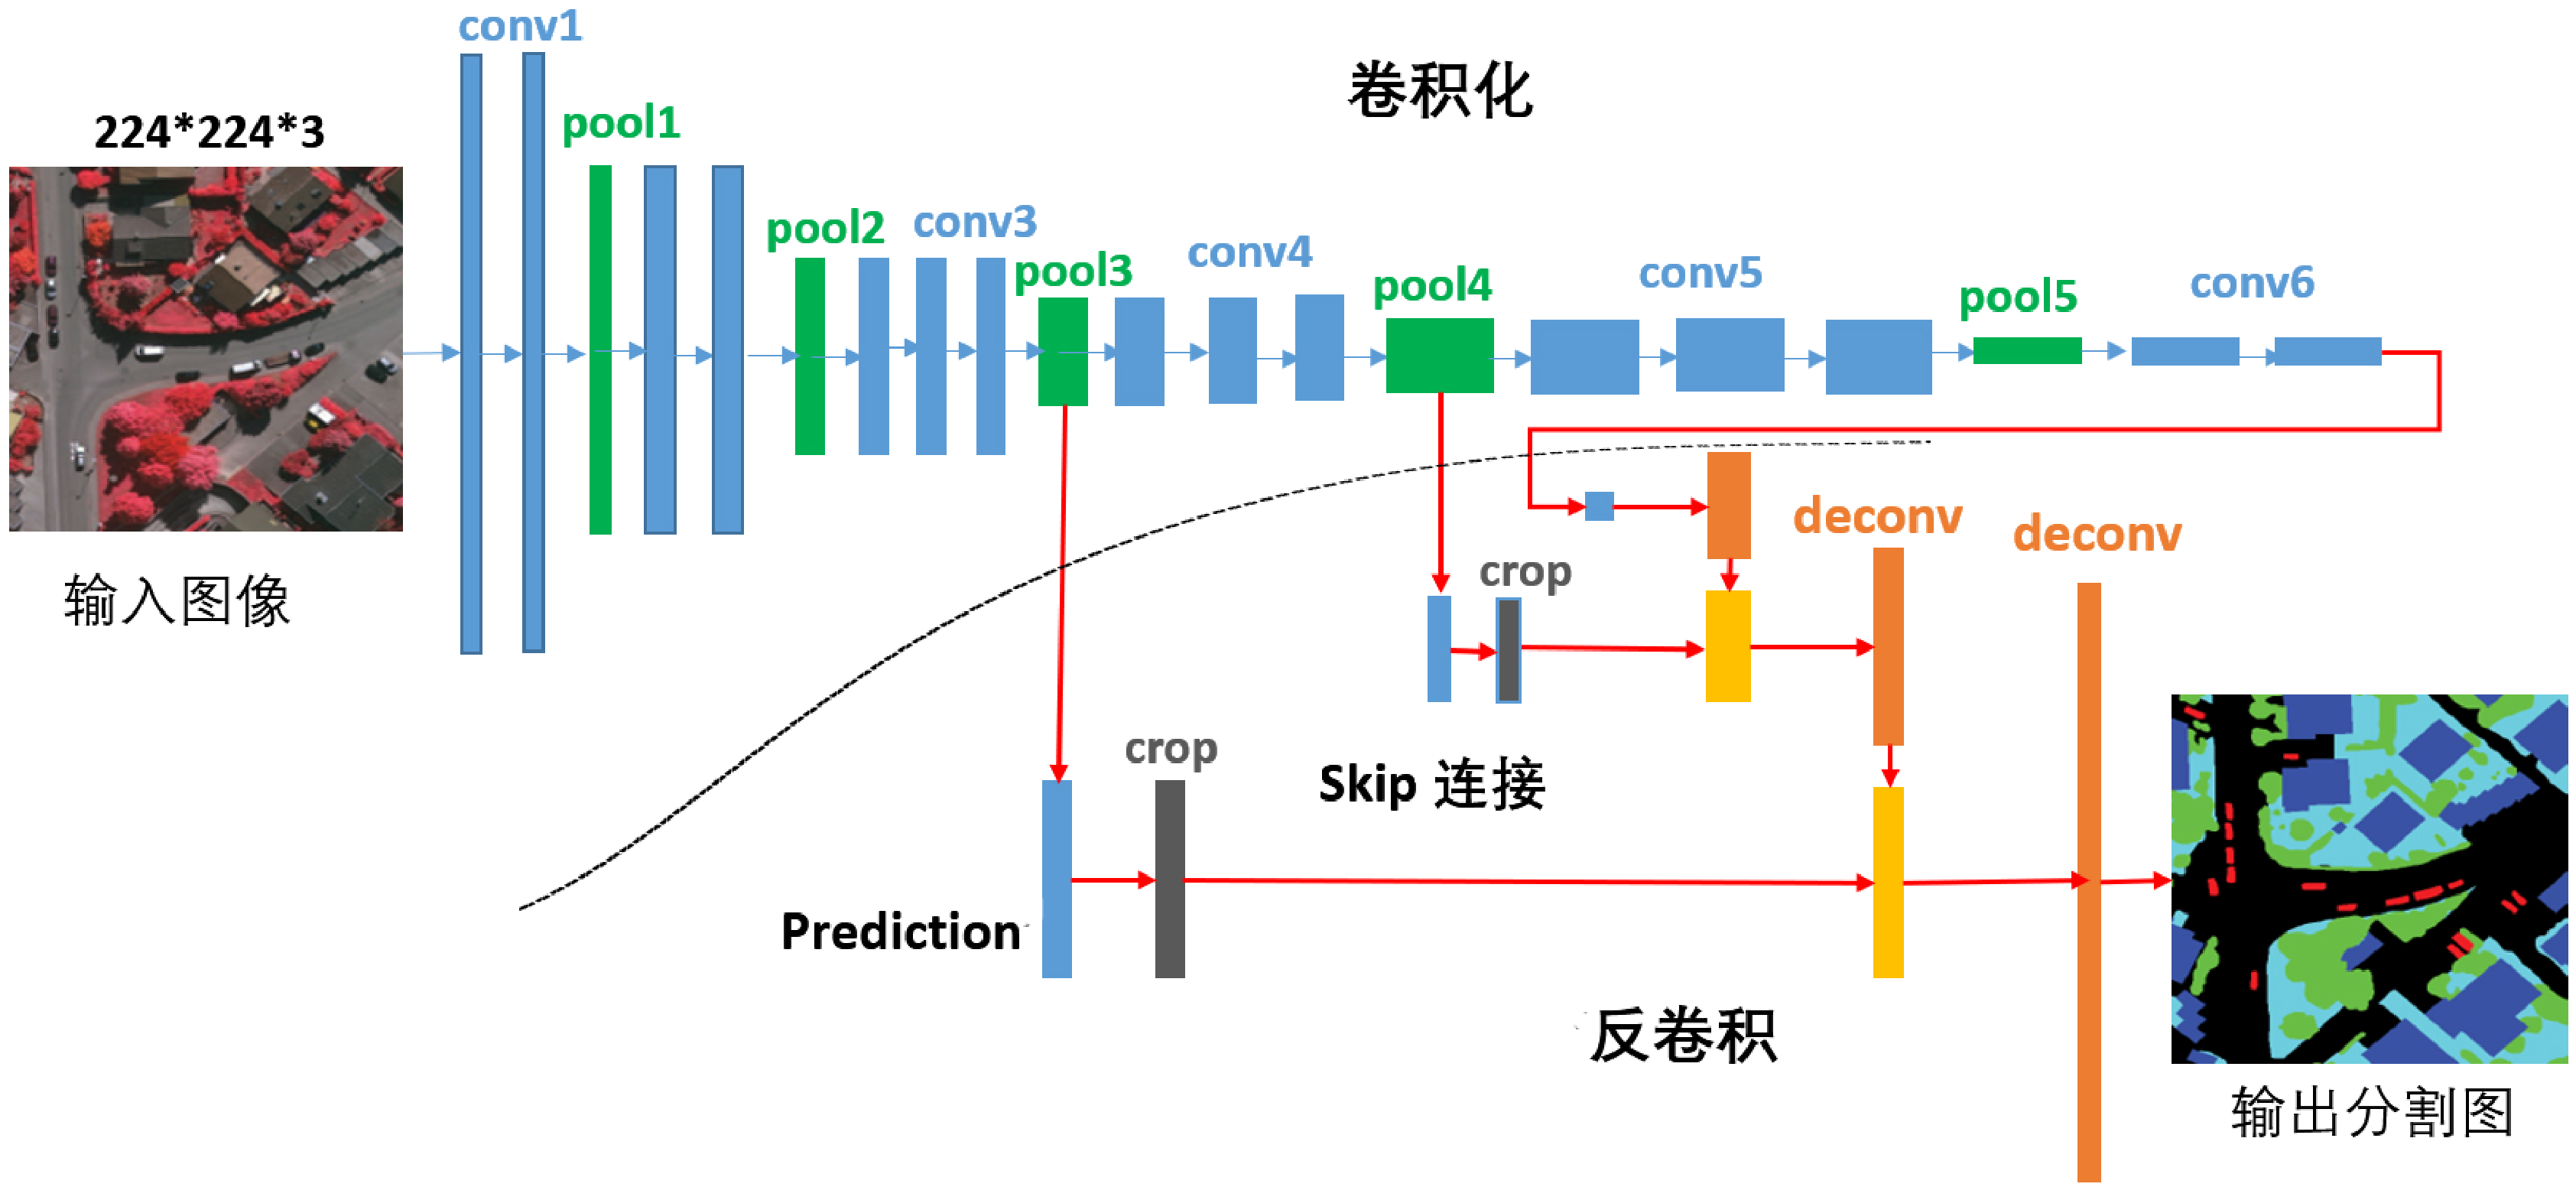
\includegraphics[width=1.0\textwidth]{figures/vgg-fcn}
  \caption{基于FCN网络的遥感影像分类示意图}\label{fig:vgg-fcn}
\end{figure}

FCN 有三个特点,分别是全卷积化、反卷积上采样和跳跃连接。全卷积化将传统CNN 网路中的全连接层全部转化为卷积层。全连接层由于神经元个数固定,与上层连接特征图的权值也是固定,从后到前一层一层地反向推导,可知CNN 模型的输入影像尺寸也必须相同,所以去除全连接层的FCN 网络可以接受任意尺寸的图像。此外,卷积操作将全连接层输出由一维映射为为二维特征矩阵,便于模型后半部分对特征图上采样处理。反卷积上采样操作能将特征图还原为原始影像大小,保留图像空间位置信息,实现影像的像素级分类。跳层连接融合卷积网络不同深度的特征输出,将影像低阶细节特征和高阶语义特征进行融合,能够得到更精细化的分类结果。

\section{生成对抗网络概述}
\label{sec:chap02-3}
前面介绍的CNN 和FCN 分类模型同属深度学习理论的判别式模型,判别式模型主要思想是根据原始样本特征决策判别样本具备的性质,例如根据影像特征判别影像包含地物所属分类。与之对应的是生成模型,生成模型是对输入数据的分布规律建立模型,进而用新模型生成样本数据。随着深度学习和神经网络近几年的迅猛发展,基于深度学习的生成模型取得了重大的突破,研究基于深度学习的生成模型也具有重大意义。2014年GoodFellow 等人从对抗博弈的角度提出一种名为生成对抗网络(Generative Adversarial Network,GAN)\cite{goodfellow2014generative} 的生成模型,该模型由生成器和判别器两部分构成。生成器试图学习潜在的数据分布规律,生成新样本;判别器则决策当前数据源为真实样本还是生成样本。相关研究\cite{mirza2014conditional}证明相比其他生成模型(如自编码网络等),GAN 生成的样本更加逼真。 

\subsection{生成对抗网络模型}
\label{sec:first-1}
GAN 模型思想启发于博弈论中的“纳什均衡”,即模型训练时不断对抗博弈,模拟数据分布的生成式模型。GAN 模型中生成器目的是生成符合数据潜在分布特征的样本,尽可能欺骗判别器;判别器目的是判断网络输入是生成样本还是真实数据,不被生成器愚弄。模型交替训练时,判别器尝试区分输入样本的来源,当判别器发现真实样本与生成样本存在差异时,模型优化生成器的权值参数,消除样本分布差异,生成器样本生成能力不断提高。而判别器优化过程则是不断提高判别器对样本的判别能力。最终模型收敛时两者达到一个“纳什均衡”,此时生成器能拟合数据的分布生成逼真样本。

\begin{figure}[htb]
  \centering
  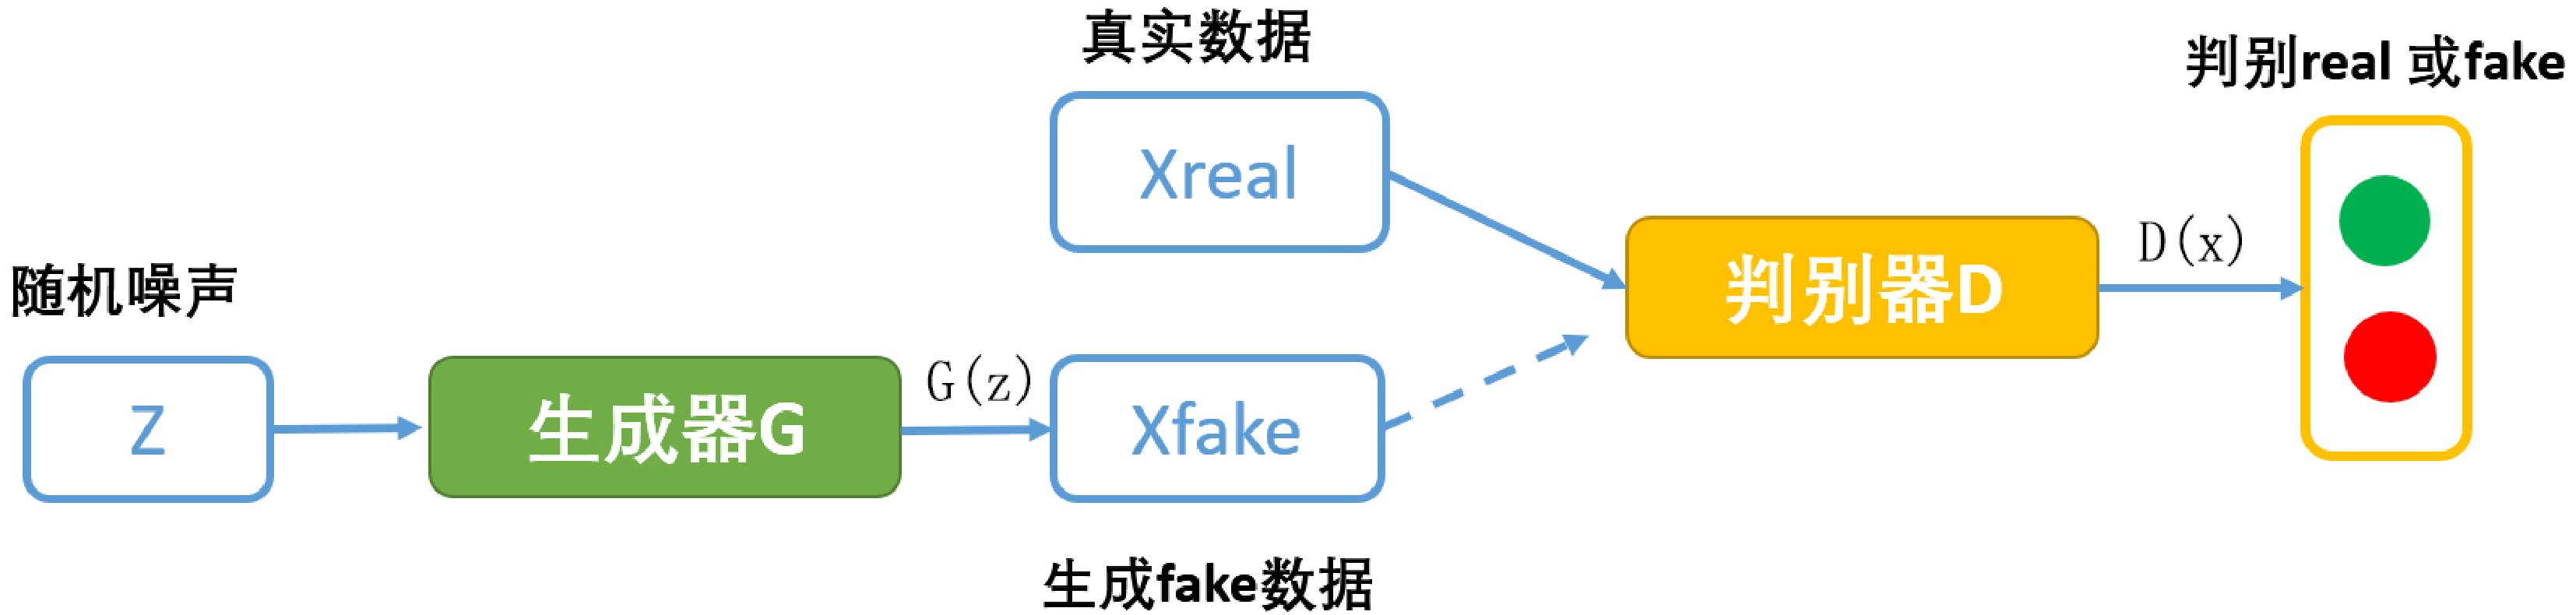
\includegraphics[width=0.8\textwidth]{figures/gan}
  \caption{GAN结构示意图}\label{fig:gan}
\end{figure}

如图\ref{fig:gan} 所示,分别用符号G 和D 表示GAN 模型生成器与判别器。假定变量$z$(通常为服从高斯分布的随机噪声)通过G 生成$X_{fake}$,D 需要决策模型输入数据是真实样本$X_{real}$还是生成的样本$X_{fake}$ 。GAN 模型需要优化的目标函数为\ref{eq:4-1}:
\begin{equation}
  \label{eq:4-1}
  \mathop{\min}_{G} \mathop{\max}_{D} V(D,G) = \mathop{\min}_{G} \mathop{\max}_{D} E_{x \sim p_{data}(x)} [\log D(x)] + E_{z \sim p_{z}(z)}[ \log (1-D(G(z)))]
\end{equation}

式中$x \sim p_{data}(x)$ 表示$x$ 取自真实的分布数据。求解D 等价于求解二分类模型,$ V(D,G)$ 即为二分类求解常见的目标代价函数。G 需要最大化生成结果的分类决策概率$D(G(z))$ 干扰D 的决策判断 ,即最小化$\log (1-D(G(z)))$ 。

模型训练时,D 和G 交替迭代训练,即先固定G 训练D,再固定D 训练G,不断迭代,直到模型收敛。对于G,最小化$\mathop{\max}_{D} V(D,G) $,即最小化$V(D,G)$ 的最大值。当固定G 时,对代价函数$V(D,G)$ 求导,解出最优的判别器$D^{\star}(x)$如式\ref{eq:4-2}:

\begin{equation}
  \label{eq:4-2}
  D^{\star}(x) = \frac{p_g(x)}{p_g(x)+p_{data}(x)}
\end{equation}

文献\cite{goodfellow2014generative} 中指出,当多次往复训练后,模型会收敛,G 与D 达到“纳什均衡”,$p_g(x) = p_{data}(x)$,即判别器对生成样本和真实样本的预测概率均为$\frac{1}{2}$, 无法区分。表明生成器已经学习到数据的内在分布,能够生成逼近真实样本的数据。


\subsection{条件生成对抗网络}
\label{sec:first-2}
经典的GAN 模型是无监督模型,其生成器的输入为随机噪声$z$,通常只能生成逼近真实样本的同类型数据,不能生成我们想要的某一种类型的数据,例如无法根据影像原始图,生成器生成影像分类结果图。文献\cite{mirza2014conditional} 针对上述问题提出条件生成对抗网络(Conditional Generative Adversarial Networks,CGAN),CGAN 模型生成器输入加入条件约束$y$ 引导模型迭代方向,即将先验条件约束$y$ 和随机噪声$z$ 联合作为生成器的输入样本,生成我们需要的目标类型数据。其中,$y$ 可以是任何种类的辅助信息,如类别标签,影像真实Ground truth 图或其他不同领域模态的数据等。

\begin{figure}[htb]
  \centering
  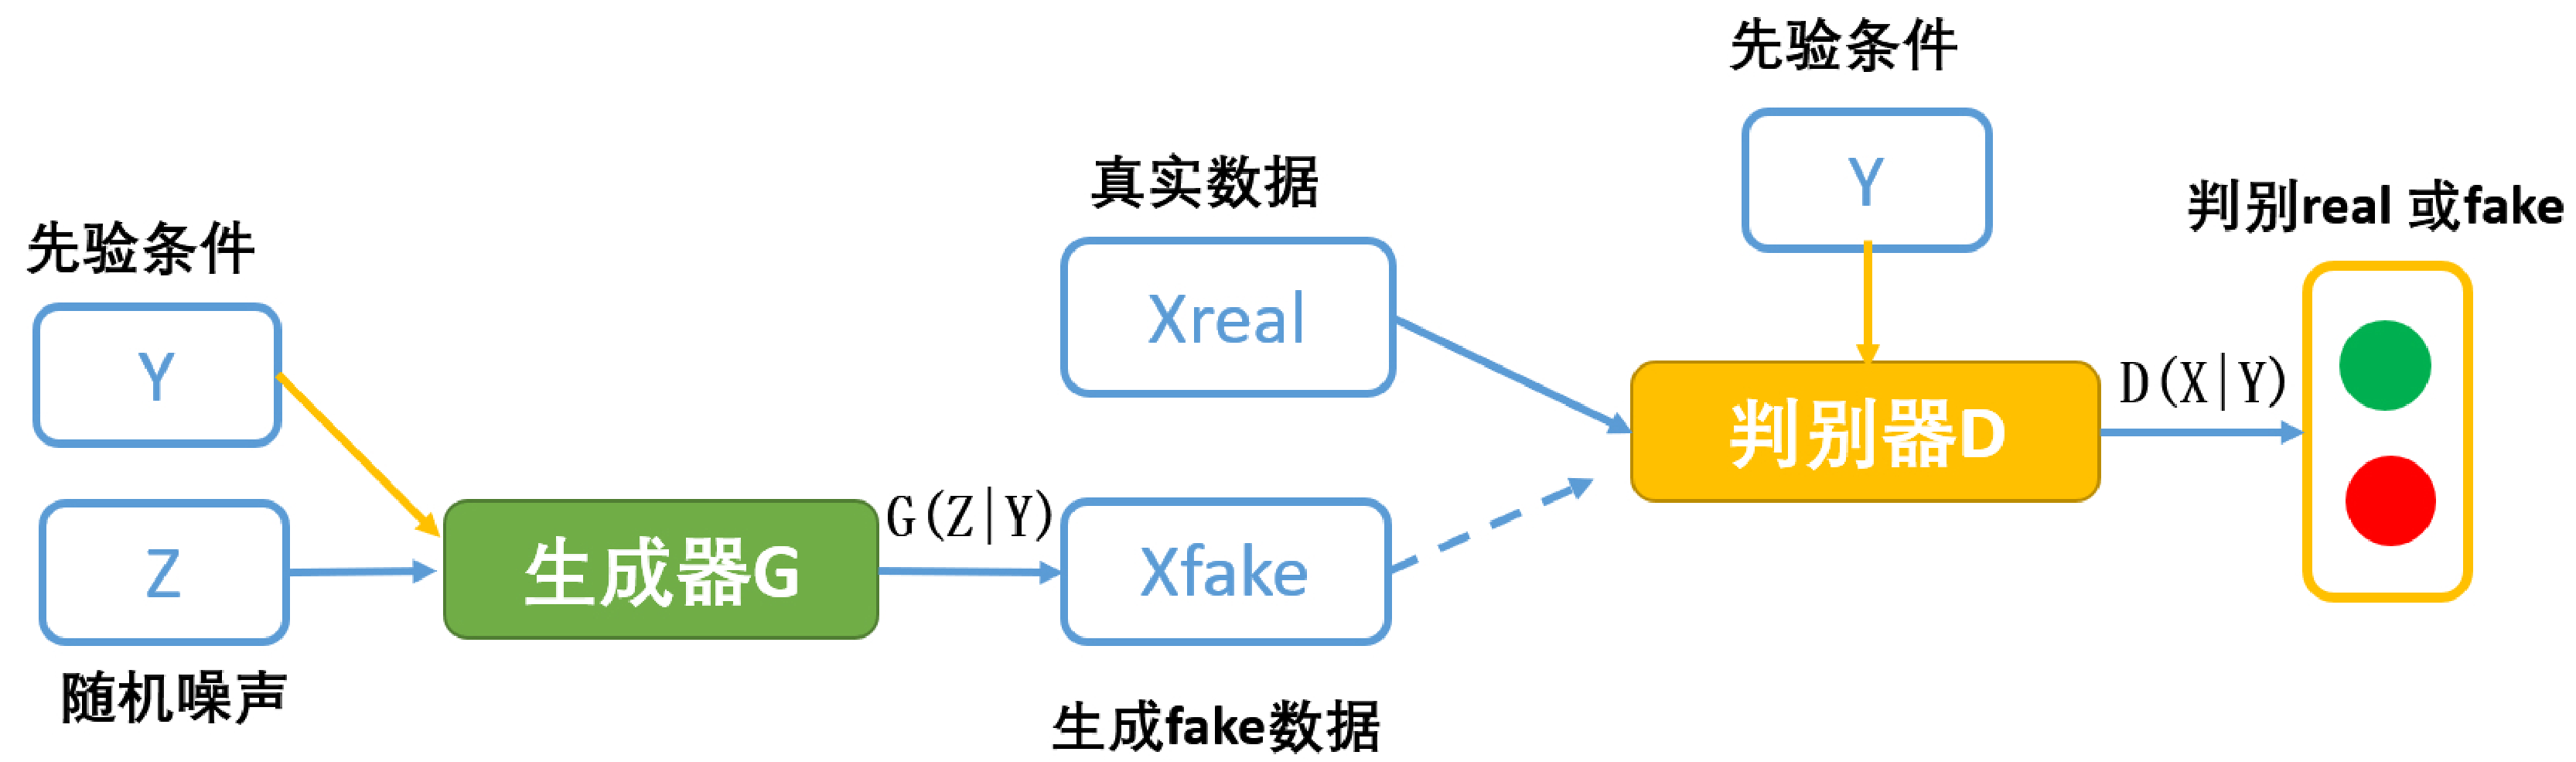
\includegraphics[width=0.8\textwidth]{figures/cgan}
  \caption{CGAN结构示意图}\label{fig:cgan}
\end{figure}

CGAN 模型中,G 中随机噪声$z$与先验知识$y$ 拼接组成G 阶段联合输入特征;D 中将真实样本/生成样本$X$ 和$y$ 通过拼接共同作为判别模型输入。 类似式\ref{eq:4-1} 中GAN 的目标函数, CGAN 模型目标函数为带有条件概率的二人极小极大值博弈函数,即:

\begin{equation}
  \label{eq:4-3}
  \mathop{\min}_{G} \mathop{\max}_{D} V(D,G) = \mathop{\min}_{G} \mathop{\max}_{D} E_{x \sim p_{data}(x)} [\log D(x|y)] + E_{z \sim p_{z}(z)}[ \log (1-D(G(z|y)))]
\end{equation}

式\ref{eq:4-3}中,$D(x|y)$ 为判别器D对有条件约束$y$ 的真实样本判别为真的代价函数,$D(G(z|y))$ 为D对有条件约束$y$ 的生成样本$G(z|y)$ 判别为假的代价函数。

图\ref{fig:cgan} 为CGAN 的结构示意图,通过将额外条件信息$y$ 分别输送给判别模型和生成模型组成联合隐层表征,作为输入层的一部分,从而指导数据的生成过程。

\section{本章小结}
\label{sec:chap02-4}

本章介绍内容为论文研究内容理论基础,围绕深度学习领域内的三大模型展开介绍。首先介绍了经典CNN 模型的结构和原理,包含CNN 卷积池化、权值共享等特性。接着介绍了FCN 模型的结构以及FCN 在遥感影像语义分割中的应用,重点介绍FCN 全卷积化与反卷积上采样的处理方式。最后,介绍了GAN 模型和带有先验约束条件的CGAN 模型的原理和结构。生成对抗网络在遥感影像分类中的应用将在后文中详细介绍。